% CVPR 2024 Paper Template; see https://github.com/cvpr-org/author-kit

\documentclass[10pt,twocolumn,letterpaper]{article}

%%%%%%%%% PAPER TYPE  - PLEASE UPDATE FOR FINAL VERSION
% \usepackage{cvpr}              % To produce the CAMERA-READY version
% \usepackage[review]{cvpr}      % To produce the REVIEW version
\usepackage[pagenumbers]{cvpr} % To force page numbers, e.g. for an arXiv version

% Import additional packages in the preamble file, before hyperref
%
% --- inline annotations
%
\newcommand{\red}[1]{{\color{red}#1}}
\newcommand{\todo}[1]{{\color{red}#1}}
\newcommand{\TODO}[1]{\textbf{\color{red}[TODO: #1]}}
% --- disable by uncommenting  
% \renewcommand{\TODO}[1]{}
% \renewcommand{\todo}[1]{#1}
\usepackage{amsthm}
\usepackage{graphicx}
\usepackage{animate}
\newcommand{\Var}{\textup{Var}}
\newcommand{\Cov}{\textup{Cov}}
\newcommand{\bE}{\mathbb{E}}
\newtheorem{proposition}{Proposition}
\newtheorem{example}{Example}


% It is strongly recommended to use hyperref, especially for the review version.
% hyperref with option pagebackref eases the reviewers' job.
% Please disable hyperref *only* if you encounter grave issues, 
% e.g. with the file validation for the camera-ready version.
%
% If you comment hyperref and then uncomment it, you should delete *.aux before re-running LaTeX.
% (Or just hit 'q' on the first LaTeX run, let it finish, and you should be clear).
\definecolor{cvprblue}{rgb}{0.21,0.49,0.74}
\usepackage[pagebackref,breaklinks,colorlinks,citecolor=cvprblue]{hyperref}


%%%%%%%%% PAPER ID  - PLEASE UPDATE
\def\paperID{00275} % *** Enter the Paper ID here
\def\confName{CVPR}
\def\confYear{2024}

%%%%%%%%% MODEL NAME
\def\modelname{LocVLM\xspace}

%%%%%%%%% TITLE - PLEASE UPDATE
\title{Learning to Localize Objects Improves Spatial Reasoning in Visual-LLMs}
% \title{Teaching Spatial Coordinates to Visual-LLMs}
% \title{Learning Image Coordinates Improves Visual-LLM Spatial Reasoning}
% \title{Spatially Aware Visual-LLM}
% \title{Spatial Awareness Improves Visual-LLM}

%%%%%%%%% AUTHORS - PLEASE UPDATE
\author{
Kanchana Ranasinghe$^{1,2}$ \quad
Satya Narayan Shukla$^1$ \quad
Omid Poursaeed$^1$ \\
Michael S. Ryoo$^2$ \quad \quad
Tsung-Yu Lin$^1$ 
\vspace{0.5em} \\ 
$^1$Meta \quad $^2$Stony Brook University 
\vspace{0.1em} \\
{\tt\small \{kranasinghe, mryoo\}@cs.stonybrook.edu, \{satyanshukla, opoursaeed, tsungyulin\}@meta.com}
% First Author\\
% Institution1\\
% Institution1 address\\
% {\tt\small firstauthor@i1.org}
% For a paper whose authors are all at the same institution,
% omit the following lines up until the closing ``}''.
% Additional authors and addresses can be added with ``\and'',
% just like the second author.
% To save space, use either the email address or home page, not both
}

\begin{document}
\maketitle

\begin{abstract}

Generative modeling aims to transform random noise into structured outputs. In this work, we enhance video diffusion models by allowing motion control via structured latent noise sampling. This is achieved by just a change in data: we pre-process training videos to yield structured noise. Consequently, our method is agnostic to diffusion model design, requiring no changes to model architectures or training pipelines. Specifically, we propose a novel noise warping algorithm, fast enough to run in real time, that replaces random temporal Gaussianity with correlated warped noise derived from optical flow fields, while preserving the spatial Gaussianity. The efficiency of our algorithm enables us to fine-tune modern video diffusion base models using warped noise with minimal overhead, and provide a one-stop solution for a wide range of user-friendly motion control: local object motion control, global camera movement control, and motion transfer. The harmonization between temporal coherence and spatial Gaussianity in our warped noise leads to effective motion control while maintaining per-frame pixel quality. Extensive experiments and user studies demonstrate the advantages of our method, making it a robust and scalable approach for controlling motion in video diffusion models. Video results are available on our \href{https://eyeline-research.github.io/Go-with-the-Flow/}{webpage}; source code and model checkpoints are available on \href{https://github.com/Eyeline-Research/Go-with-the-Flow}{GitHub}.

\end{abstract}    
\section{Introduction}
\label{locVLM_sec:intro}

Holistic visual understanding requires learning beyond simply content of an image to encompass awareness on spatial locations of objects and their relations \cite{marr1982vision}. In the context of visual question answering (VQA), such spatial awareness allows better reasoning involving structural and contextual information contained within an image \cite{chen2023shikra}.

Since the introduction of powerful large-language models (LLMs) such as GPT-3 \cite{brown2020language}, Chat-GPT \cite{gpt4}, Vicuna \cite{vicuna2023}, and LLaMA~\citep{touvron2023llama,touvron2023llama2} that are capable of human style conversation, their visual counterparts such as BLIP-2 \cite{li2023blip}, LLaVA \cite{liu2023visual} have enabled novel tasks within the vision modality. However, despite their \cite{li2023blip,liu2023visual} highly generic visual understanding, these models exhibit poor language-based spatial reasoning \cite{chen2023shikra}. In fact, they fail at simple tasks such as distinguishing whether an object lies to the left or right of another object (see \cref{locvlm_tbl:spatial_icl}). 
% half of the image

\begin{figure}[t]
\centering

\includegraphics[width=.5\linewidth]{figures__intro1.png}\\
\texttt{man with blonde hair in blue shirt and brown pants}

\includegraphics[width=.5\linewidth]{figures__intro2.png}\\
\texttt{bald man wearing glasses with white shirt and black pants}

\caption{\textbf{Zero-Shot Segmentation with phrases}:  We highlight the ability of \modelname to ground complex language prompts onto an image with no segmentation specific training. An off-the-shelf diffusion model is used with only an inference time optimization technique to generate these segmentations. If you look closely, you'll notice the bald man's arms are segmented - but are not visible in the photo! Peekaboo has fairly strong shape priors.}
\label{fig:intro}
\end{figure}


In the case of contrastive language image models (such as CLIP \cite{radford2021learning}, ALIGN \cite{Jia2021ScalingUV}), recent works explore how injecting explicit spatial awareness \cite{Zhang2023AssociatingSG,Luo2022SegCLIPPA,Mukhoti2022OpenVS,Ranasinghe2022PerceptualGI} can enable more holistic visual understanding. In fact, \cite{Ranasinghe2022PerceptualGI} shows how such improved spatial awareness benefits model robustness in adversarial domains. 
This raises the question of how generative language image models, particularly those connecting LLMs to visual encoders \cite{li2023blip,liu2023visual} can benefit from such spatial awareness specific training. We refer to models of this category that generate textual outputs given joint image-text inputs (e.g. \cite{li2023blip,liu2023visual}) as visual-LLMs (V-LLMs). 

In this work, we explore location specific instruction fine-tuning objectives that explicitly enforce V-LLMs to meaningfully process and generate textual image-space coordinates. We hypothesize that such training would lead to improved spatial awareness in these V-LLMs, therein improving performance on VQA tasks. To this end, we propose three instruction fine-tuning objectives that unify location representation with natural language. We also explore optimal representation forms for image-space locations and how pseudo-data generation can be leveraged for efficient scaling of our framework. We name our resulting model as LocVLM.  

While the idea of adapting V-LLMs to perform localization related tasks (e.g. detection, segmentation) using V-LLMs has been explored in multiple recent works \cite{zhang2023gpt4roi,zhao2023bubogpt,zang2023contextual,peng2023kosmos,You2023FerretRA,wang2023visionllm,lai2023lisa}, these approaches depend on task specific architectural modifications or treat localization inputs / outputs differently from natural language. In contrast, our LocVLM focuses on a unified framework treating location and language as a single modality of inputs with the goal of complementing performance in each task. We intuit that processing location represented in textual form would enforce the LLM to select appropriate image regions as opposed to relying on region level features provided by the architecture. At the same time, textual form location outputs promote spatial awareness at language level in a human interpretable manner, in contrast to using secondary heads or specialized tokens for location prediction.  
Concurrent work in \cite{chen2023shikra} also explores textual location representation with a generic V-LLM architecture similar to our work. Our proposed LocVLM differs with focus on optimal location representation forms, data-efficient pseudo-labelling, and video domain operation. 

Our proposed framework exhibits improved spatial awareness in VQA style conversation demonstrated through experimentation on 14 datasets across 5 vision-language tasks: Spatial Reasoning, Image VQA, Video VQA, Object Hallucination, and Region Description. 
We summarize our key contributions as follows: 
\begin{itemize}[leftmargin=2em,noitemsep,topsep=0.0ex,itemsep=-1.0ex,partopsep=0ex,parsep=1ex]
    \item Inject textual spatial coordinate awareness into V-LLMs 
    \item Propose three novel localization based instruction fine-tuning objectives for V-LLMs 
    \item Discover optimal coordinate representation forms 
    \item Pseudo-Data generation for improved region description and scaling to video domain
\end{itemize} 

\section{Spatial Reasoning in Visual-LLMs}
\label{locvlm:related}

\noindent
\textbf{Localization in Contrastive Vision Language Models}:
Foundation vision language models (VLMs) such as CLIP \cite{radford2021learning} resulted in extensive exploration into language-tied localization in images both under dense (pixel / bounding-box) supervision \cite{gu2021vild, kamath2021mdetr, Li2022AdaptingCF, Li2021GroundedLP, Zeng2021MultiGrainedVL,Dou2022CoarsetoFineVP,ghiasi2022open, li2022language, Zhang2022GLIPv2UL,Ding2021DecouplingZS} and weak supervision \cite{xu2022groupvit, Xu2023LearningOS, Zhou2021ExtractFD, yao2022filip,cui2022democratizing, Zhang2023AssociatingSG,Luo2022SegCLIPPA,Ranasinghe2022PerceptualGI,Mukhoti2022OpenVS}. Recovering explicit localization information within model representations has enabled more robust operation for certain tasks \cite{Ranasinghe2022PerceptualGI}. While our work differs from this contrastive setting given our use of LLM based generative predictions, we similarly explore how explicit location information within the language modality can improve V-LLMs.  

\vspace{0.5em}

\noindent
\textbf{Visual Large Language Models (V-LLMs)}:
The advent of powerful large language models (LLMs) such as GPT-3 \cite{brown2020language}, Chat-GPT \cite{gpt4}, and PaLM \cite{chowdhery2022palm}, as well as their open-source counterparts BLOOM~\citep{scao2022bloom}, Vicuna \cite{vicuna2023}, and LLaMA~\citep{touvron2023llama,touvron2023llama2}, has resulted in direct use of these LLMs for computer vision tasks \cite{Gupta2022VisualPC, Suris2023ViperGPTVI}. Alternate lines of work explore how LLMs can be connected to existing visual foundation models \cite{alayrac2022flamingo,anas_awadalla_2023_7733589,Ranasinghe2023LanguagebasedAC,li2023blip,liu2023visual,Maaz2023VideoChatGPT}, in particular to CLIP visual backbones \cite{radford2021learning}. While earlier models explored large-scale (millions to billions of samples) image-text training \cite{alayrac2022flamingo,anas_awadalla_2023_7733589}, later models \cite{li2023blip,liu2023visual,Maaz2023VideoChatGPT} scale down on data dependency. LLaVA \cite{liu2023visual} in particular scales down on pre-training data to under 1 million image-text pairs, and use instruction fine-tuning \cite{Wei2021FinetunedLM} to enable human-style conversation with visual awareness. This is extended to video domain in \cite{Maaz2023VideoChatGPT,ranasinghe2024understanding}. A shortcoming of these models is their lack of spatial awareness or location understanding in image space \cite{chen2023shikra,Gokhale2022BenchmarkingSR,Cho2022DALLEVALPT}.
% - in our work we attempt to address this limitation. 
Spatial reasoning limitations in generative VLMs are studied in \cite{Gokhale2022BenchmarkingSR,Cho2022DALLEVALPT}. Similar failures in captioning (and VQA) models are explored in \cite{Kamath2023WhatsW}. A solution in \cite{Hsu2023WhatsLC} proposes code-generation based reasoning. Our work tackles these same limitations but follows an alternate direction of spatial-aware instruction fine-tuning.
Another line of recent works \cite{zhang2023gpt4roi,zhao2023bubogpt,zang2023contextual,peng2023kosmos,You2023FerretRA,wang2023visionllm,lai2023lisa} tackle this by introducing architectural modifications to explicitly extract region level features that are injected to the LLM as special tokens. While introducing extra tokens and layers, this also separates the localization task from language. 
In contrast, we use a generic architectures with purely textual location information (i.e. image space coordinates as text).  
% We postulate that generic architectures with purely language driven location information (i.e. reasoning in image coordinate space) would inject LLMs with stronger spatial awareness more similar to human visual understanding and reasoning. 
Concurrent work in \cite{chen2023shikra} explores this same idea, but we differ in 3 ways with, a) focus on optimal coordinate representation forms, b) data-efficient pseudo-labelling strategies, and c) video domain operation (see also \cref{tbl:related}). 

\begin{table}[t]
\centering
\small
\def\arraystretch{1.0}  % height
\setlength\tabcolsep{0.5em}  % width
\scalebox{0.95}{
\begin{tabular}{l|c|c|c|c}
\toprule
Method          & Kosmos \cite{peng2023kosmos} & Ferret \cite{You2023FerretRA} & Shikra \cite{chen2023shikra} & Proposed \\ \midrule
Unified Arch.   & \xmark & \xmark & \cmark & \cmark  \\ 
Purely Textual  & \xmark & \xmark & \cmark & \cmark  \\ 
Pseudo Data     & \xmark & \xmark & \xmark & \cmark  \\ 
Video Domain    & \xmark & \xmark & \xmark & \cmark  \\ \bottomrule
\end{tabular}
}
\vspace{-0.5em}
\caption{Related Work Comparison: 
% We highlight key distinctions of our proposed method against three most similar related works. 
A unified architecture, purely textual inputs, pseudo data for scalable learning, and video domain operation distinguishes our proposed work from these prior methods.}
\label{tbl:related}
\end{table}

\vspace{0.5em}
\noindent
\textbf{Location Representations}:
Selecting regions within an image has a rich history in computer vision \cite{malik2001visual,uijlings2013selective} with greater focus on location outputs since the popularity of object detection \cite{girshick2015fastrcnn, redmon2016yolo, tian2019fcos, carion2020detr, chen2022diffusiondet, chen2021pix2seq, wang2023visionllm}. Early anchor-based methods regress locations from anchor centers \cite{girshick2015fastrcnn, redmon2016yolo}, followed by direct location regression from object-level features \cite{tian2019fcos, carion2020detr}. Recent works explore generative location predictions with diffusion processes \cite{chen2022diffusiondet} and sequence-generation \cite{chen2021pix2seq, wang2023visionllm}. Ours resembles the latter given our use of an LLM, next token prediction objective, and sequential generation of textual location representations. However, \cite{chen2021pix2seq, wang2023visionllm} utilize 1000 specialized location tokens (introduced to the LLM vocabulary) corresponding to 1000 bins uniformly spread across image space. While we explore similar binning strategies, in contrast we introduce no additional tokens, focus on purely textual representation of locations, and explore multiple textual location representation forms.  


\section{Method}
\label{sec:method}

\method is comprised of two separate parts: our noise warping algorithm and video diffusion fine-tuning. The noise warping algorithm operates independently from the diffusion model training process: we use the noise patterns it produces to train the diffusion model. Our motion control is based \textit{entirely} on noise initializations, introducing no extra parameters to the video diffusion model.

Inspired by the existing noise warping algorithm HIWYN~\cite{chang2024warped}, which introduced noise warping for image diffusion models, we introduce a new use case for the warped noise: we use it as a form of \textit{motion conditioning} for video generation models. After fine-tuning a video diffusion model on a large corpus of videos paired with warped noise, we can control the motion of videos at inference time.

\subsection{\method noise warping}

% algorithm placeholder
\begin{algorithm}[t]
\caption{\method next-frame warping}
\label{alg:main}
\begin{algorithmic}[1]
\State \textbf{Input:} previous-frame noise $q \in \mathbb{R}^{D}$, previous-frame density $p \in \mathbb{R}^{D}$, forward flow $f: D \to \mathbb{N}^2$, backward flow $f': D \to \mathbb{N}^2$.
\State Let $G = (V, V', E)$ be a bipartite graph with $V = D$, $V' = D$ and edge set $E = \{\}$ to be constructed. % this is really unecessary: \Comment{$E$ only contains edges from $V$ to $V'$.}
\For{$v$ in $V$} \Comment{Contraction}
\State $E \gets E \cup (v, v+f(v))$ if $v+f(v')\in D$
\EndFor
\For{$v'$ in $V'$} \Comment{Expansion}
\If{$\deg_G(v') = 0$} \Comment{$\deg_G(v)$ denote the degree of $v$ in $G$}
\State $E \gets E \cup (v' + f'(v'), v')$ if $v' + f'(v')\in D$
\EndIf
\EndFor
\For{$v$ in $V$} \Comment{Conditional white noise sampling}
\State $d \gets \deg_G(v)$
\State Sample $Z \sim \mathcal{N}(0, I_{d})$, and set $S \gets \sum_{i=1}^d Z_i$
\State $X_i \gets \frac{q(v)}{d} + \frac{1}{\sqrt{d}}(Z_i - \frac{S}{d})$ for $i \in [d]$
\State $R(v) \gets \{X_i\}_{i\in[d]}$ 
\EndFor
\For{$(v')$ in $V'$} \Comment{Compute next-frame noise and density}
\State $q'(v') \gets 0$, $p'(v') \gets 0$, $s \gets 0$
\For{{$v$ in $V$ such that $(v,v') \in E$}}
\State $d \gets \deg_G(v)$, $\alpha \gets \frac{p(v)}{d}$
\State $q'(v') \gets q'(v') + \alpha R(v)\text{.pop}()$
\State $p'(v') \gets p'(v') + \alpha$
\State $s \gets s + \alpha^2 \frac{1}{d}$
\EndFor
\If{$s = 0$}
\State Sample $q'(v') \sim \mathcal{N}(0, 1)$
\Else
\State $q'(v') \gets \frac{q'(v')}{\sqrt{s}}$ \Comment{Renormalize to unit variance}
\EndIf
\EndFor
\State \textbf{return} next-frame noise and density $q', p'$.
\end{algorithmic}
\label{alg:algorithm}
\end{algorithm}


\subsubsection{Algorithm}


To facilitate the large-scale noise warping required by this new use case, we introduce a fast noise warping algorithm (\cref{alg:main}) that warps noise frame-by-frame, storing just the previous frame's noise (with dimensions $H \times W \times C$, where $H$ is height, $W$ is width, and $C$ is the number of channels) and a matrix of per-pixel flow density values (with dimensions $H \times W$). The density values indicate how much noise has been compressed into a given region. Unlike HIWYN~\cite{chang2024warped} which requires time-consuming polygon rasterization and upsampling of each pixel, our algorithm directly tracks the necessary \textit{expansion} and \textit{contraction} between frames according to the optical flow and uses only pixel-level operations that are easily parallelizable. We show that our algorithm retains the same Gaussianity guarantee as HIWYN~\cite{chang2024warped} (\cref{prop:gaussianity}).

\noindent \textbf{Next-frame noise warping}. Our noise warping algorithm calculates noise iteratively, where the noise for a given frame depends only on the state of the previous frame.

Let $H\times W$ be the dimensions of each video frame. Let $D = [H]\times [W]$ denote a 2D matrix with height $H$ and width $W$, where we use the notation $[n]:= {1,\ldots, n}$. Given the previous frame's noise\footnote{Since different channels are treated independently, we will assume a single channel in images.} $q \in \mathbb{R}^D$ and the flow density $p \in \mathbb{R}^D$ together with forward and backward flows\footnote{We allow flows to go out of bounds, i.e., $f$ and $f'$ can land in $\mathbb{N}^2 \setminus D$.} $f,f':D\to \mathbb{N}^2$, our algorithm computes the next-frame noise and density $q',p' \in \mathbb{R}^D$ such that $q'$ (resp. $p'$) is temporally correlated with $q$ (resp. $p$) via the flows.

At a high level, our algorithm (in~\cref{alg:algorithm}) combines two types of dynamics: \textit{expansion} and \textit{contraction}. In the case of \textit{expansion}, such as when a region of the video zooms in or an object moves towards the camera, one noise pixel is mapped to one or more noise pixels in the next frame (hence it ``expands''). In the case of \textit{contraction}, we adopt the Lagrangian fluid dynamics viewpoint of treating noise pixels as particles moving along the forward flow $f$. This often leaves gaps that need to be filled. Hence, for regions not reached when flowing along $f$, we use the backward flow $f'$ to pull back a noise pixel. That gap is filled with noise calculated with the \textit{expansion} case.

Additionally, to preserve the distribution correctly over long time periods, we use density values to keep track of how many noise pixels were aggregated into a given region, so that when mixed with other nearby particles in the \textit{contraction} case, these higher density particles have a larger weight. This is illustrated in \cref{fig:algorithm_diagram}.

We unify both \textit{expansion} and \textit{contraction} cases by building a bipartite graph $G$ where edges represent how noise and density should be transferred from the previous frame to the next. When aggregating the influence from graph edges to form the next-frame noise $q'$, we scale the noise in accordance with the flow density to ensure the preservation of the original frame's distribution, as detailed in ~\cref{alg:algorithm}. The \textit{expansion} and \textit{contraction} cases are calculated in tandem to prevent any cross-correlation, guaranteeing the output will be perfectly Gaussian.


\subsubsection{Theoretical analysis}

\begin{figure}
    \centering
    \includegraphics[width=\linewidth]
    {fig/algo_diagram_2_layers.png}
    \caption{Diagram of our noise warping algorithm. A case example of our algorithm illustrates both the \textit{expansion} and \textit{contraction} cases, along with example density values. Each node represents some noise pixel `q'. Noise values $q_{0..3}$ are transferred from frame 0 to frame 1 using forward optical flow, and the remaining pixels in frame 1 that did not receive any values obtain their values from frame 0 using reverse optical flow (the \textit{expansion} case). In the \textit{contraction} cases such as $q'_2$, their densities become the sum of their sources. And in the \textit{expansion} case, where one source pixel spreads out into multiple target pixels, such as $q_2$ spreading out into $q'_1$ and $q'_3$, its density is dispersed.}
    \label{fig:algorithm_diagram}
\end{figure}

\begin{proposition}[Preservation of Gaussian white noise]
\label{prop:gaussianity}
If the pixels of the previous-frame noise $q$ in \cref{alg:main} are i.i.d. standard Gaussians, then the output next-frame noise $q'$ also has i.i.d. standard Gaussian pixels. Please check the appendix for a formal mathematical proof.
\end{proposition}

\begin{proposition}[Time Complexity]
\label{prop:time_complexity}
For a given frame, the time complexity of this algorithm is  $O(D)$, linear time with respect to the number of noise pixels processed. Proof: There are only two cases - \textit{contraction} and \textit{expansion}. Because each previous-frame pixel can only be contracted to one current-frame pixel, and during \textit{expansion} each current-frame pixel can only be mapped to one previous-frame pixel, the total number of edges $E$ will never exceed $2D$.
\end{proposition}

\subsection{Training-free image diffusion models with warped noise}

As shown by \citet{chang2024warped} and \citet{deng2024infinite}, noise warping can be combined with image diffusion models to yield temporally consistent video edits without training. To do this, we first take an input video and calculate its optical flows using RAFT~\cite{teed2020raft}. Then, with~\cref{alg:algorithm}, we use the flow fields to create sequences of Gaussian noise for each frame in the input video, ensuring that the noise moves along the flow fields. These noises are used during the per-frame diffusion processes in place of what would normally be temporally independently sampled Gaussian noise. This enables temporally consistent inference for video tasks, such as relighting~\cite{he2024diffrelight} and super-resolution~\cite{stabilityai2023deepfloyd}, using image-based diffusion models.

\begin{figure*}
    \centering
    \includegraphics[width=\linewidth]{fig/degradation_comparison.png}
    \caption{Showcasing the effect of noise degradation level $\deglevel$ on generated videos. A few frames from the driving video are shown in the leftmost column. Our model outputs are in the next 3 columns. As degradation decreases ($\deglevel$ from 0.7 to 0.5), the video more strictly adheres to the input flow. This allows us to control video movement with a user-specified level of precision.}
    \label{fig:degredation_lions}
\end{figure*}

\subsection{Fine-tuning video diffusion models with warped noise}

We use warped noise to condition a video diffusion model on optical flow. In particular, we fine-tune two variants of a latent video diffusion model CogVideoX~\cite{yang2024cogvideox}, both the text-to-video (T2V) and image-to-video (I2V) variants. We regard CogVideoX as a black box without changing its architecture.

We use the same training objective as in normal fine-tuning, i.e., the mean squared loss between denoised samples and samples with noise added. In fact, we use the exact same training pipeline as the original CogVideoX repository, with exactly one difference: during training, we use warped noise instead of regular Gaussian noise. For each training video, we calculate its optical flow for each frame, and create a warped noise tensor $\mathbf{Q} \in \mathbb{R}^{F \times C \times H \times W}$, where $F, C, H, W$ are the number of frames, the number of channels, the height and width of encoded video samples respectively by applying our algorithm iteratively.

We also introduce the concept of noise degradation, which lets us control the strength of our motion conditioning at inference time. After calculating the clean warped noise, we then degrade it by a random degradation level $\deglevel \in [0,1]$, by first sampling uncorrelated gaussian noise $\zeta \sim \mathcal{N}(0, 1)$ and modifying the warped noise $\Q \gets \frac{(1 - \deglevel) \Q + \zeta \deglevel}{\sqrt{(1 - \deglevel)^2 + \deglevel^2}}$. As degradation level $\deglevel \rightarrow 1$, $\Q$ approaches an uncorrelated Gaussian, and as $\deglevel \rightarrow 0$, $\Q$ approaches clean warped noise. At inference, the user can control how strictly the resulting video should adhere to the input flow. Please see \cref{fig:degredation_lions} for a qualitative depiction of the effect of $\deglevel$.

In practice, because the diffusion model works on latent embeddings, we calculate the optical flow and warped noise in image space and then downsample that noise into latent space, which in the case of CogVideoX means downscaling by a factor of $8\times8$ spatially and $4$ temporally. We use nearest-neighbor interpolation along the temporal axis and mean-pooling along the two spatial axes, which are then multiplied by $8$ to preserve unit variance.

\subsection{Video diffusion inference with warped noise}

At inference, we generate warped noise from an input video to guide the motion of the output video. Then, using a deterministic sampling process such as DDIM \cite{song2021denoising}, we use that warped noise to initialize the diffusion process of our fine-tuned video diffusion model. This method of control is much simpler than other motion control methods, as it does not require any changes to the diffusion pipeline or architecture - using exactly the same amount of memory and runtime as the base model.

In the case of local object motion control, we allow the user to specify object movements through a simple user interface as shown in~\cref{fig:comparisons_video_diffusion_object_motions}. It is used to generate synthetic optical flows, where multiple layers of polygons are overlaid on an image. Then, these polygons are translated, rotated and scaled with paths defined by the user. We warp the noise accordingly, and use that noise to initialize the diffusion process, along with a text prompt, and in the case of the image-to-video model, a given first frame image. By controlling the extent to which the output video follows these polygons, users can simulate camera movement by shifting the background, or even 3D motion effects by overlaying two polygons in parallax and moving them at different speeds. We find that this motion control representation is quite robust to user error, where even if the polygon only roughly matches the object or area of interest it will still produce high quality results. For synthetic object motion control, we typically use a degradation value $\deglevel$ between 0.5 and 0.7, depending on the level of motion precision the user desires, which is a higher level than we would normally use for motion transfer.

The case of motion transfer and camera motion control are very similar -- the only difference is the source of the flows used to generate the warped noise. In the case of motion transfer, we calculate the optical flow of a driving video, get warped noises that match the motion. Like in local object motion control, we use that warped noise to initialize a diffusion process. In the case of motion transfer, we typically use a lower degradation value $\deglevel$ between 0.2 and 0.5, as we usually want the output video's motion to match the driving video's motion as closely as possible.

\subsection{Implementation details}

We fine-tune the recent state-of-the-art open-source video diffusion model, CogVideoX-5B~\cite{yang2024cogvideox}, on both its T2V and I2V variants. We use a large general-purpose video dataset composed of 4M videos with resolution $\geq$720$\times$480 ranging from approximately 10 to 120 seconds in length, with paired texts captioned by CogVLM2~\cite{wang2024cogvlmvisualexpertpretrained}. We used 8 NVIDIA A100 80GB GPUs over the course of 40 GPU days, for 30,000 iterations using a rank-2048 LoRA~\cite{hu2021loralowrankadaptationlarge} with a learning rate of $10^{-5}$ and a batch size of 8.

Our method is data agnostic and model agnostic. It can be used to add motion control to arbitrary video diffusion models, while only processing the noise sampling during fine-tuning. For example, it also works with AnimateDiff \cite{guo2024animatediff} fine-tuned with the WebVid dataset~\cite{Bain21}, trained on 8$\times$40GB A100 GPUs over a period of 2 days with 12 frames and $256\times320$ resolution. See its qualitative results in \cref{fig:supp_animatediff_grid} in the supplementary material.
\section{Experiments}
\label{locvlm_sec:exp}

In this section, we present experimental results to highlight existing weaknesses of SOTA V-LLMs and how our proposed framework addresses these issues. We also evaluate on standard VQA benchmarks across domains to showcase the better reasoning abilities of our model and highlight novel abilities of our framework. 

\subsection{Experimental Setup}
\label{locvlm_subsec:exp_setup}
\textbf{Datasets}: 
We utilize the COCO dataset \cite{lin2014microsoft} and our model (post stage one training) to construct a localization related VQA dataset as outlined in \cref{locvlm_subsec:train_obj,locvlm_subsec:pseudo}. We name this dataset \textit{Localize-Instruct-200K}. In detail, this contains LocPred and RevLoc question-answer pairs that use pseudo-captions instead of COCO categories as well as NegPred. We define a second video dataset, \textit{Localize-ActivityNet}, containing question-answer pairs constructed from Activity-Net pseudo-bounding boxes following \cref{locvlm_subsec:video}. 
Our models are primarily trained on our Localize-Instruct-200K dataset. Our stage one training uses CC3M dataset \cite{Changpinyo2021Conceptual1P}. 
% LLaVA-Instruct-80K dataset from \cite{liu2023visual}. 
Additionally, our Localize-ActivityNet dataset and ActivityNet dataset \cite{Heilbron2015ActivityNetAL} are used for video domain training. 

\noindent \textbf{Training}: We train our models on 8xA100 GPUs (each 80GB) following a two-phase training schedule. Our first phase trains on CC3M \cite{Changpinyo2021Conceptual1P} following the setup in \cite{liu2023visual}. 
The second phase uses our Localize-Instruct-200K dataset and trains for 10 epochs with a batch size of 64, ADAM-W optimizer with initial learning rate $2e-5$, 0.3 warm-up ratio, and cosine-decay learning rate schedule. 
% The third phase uses our Localize-Instruct-200K dataset jointly with LLaVA-Instruct-80K dataset \cite{liu2023visual} to train for 1 epoch (with all other settings identical to phase two). 
Both the training phases we conduct use standard next-token-prediction loss used in LLM training. 

\noindent \textbf{Evaluation}: During evaluation, following standard protocol \cite{liu2023visual}, we iteratively generate next tokens, given visual and textual inputs. The LLM output is a distribution across the entire token vocabulary. The next token is selected through multinomial sampling of this output using a softmax temperature term of 0.2 during normalization. 


\subsection{Spatial Reasoning: A Toy Experiment}
\label{locvlm_subsec:spatial}
We investigate spatial reasoning abilities of two SOTA V-LLMs, LLaVA \cite{liu2023visual} and BLIP-2 \cite{li2023blip}, using a simple toy experiment. We create an evaluation dataset from COCO annotations containing images with distinct category object triplets (only one instance occurrence of each object category), where each object is entirely to the left or right half of the image and two objects are on opposite sides. 
The ground-truth bounding box annotation are utilized to automate this dataset creation procedure. 
This evaluation set, referred as \textit{COCO-Spatial-27K}, contains 26,716 image-question pairs (see \cref{locvlm_supp:dataset} for details). 
We introduce two evaluation settings, direct VQA and in-context learning (ICL) VQA to understand spatial reasoning abilities of these models. In direct VQA, given an image we query the model whether an object lies above or below another object. In ICL VQA, before a similar final query, we provide two example question-answer pairs (involving the other two objects in the image) in the same format as our query. 
Refer to \cref{locvlm_supp:toy} for further details on task. We perform the same for objects in top vs bottom halves of images. 

These results are presented in \cref{locvlm_tbl:spatial_icl}. Our results indicate near random performance for existing V-LLMs. 
% that are instruction fine-tuned on question answer data. 
For the case of LLaVA, we perform keyword (\textit{left} and \textit{right}) frequency analysis on its instruction tuning dataset (LLaVA-Instruct-80K dataset) to verify the presence of terms \textit{left} and \textit{right} in its training corpus. These keywords are present in 0.37\% and 1.13\% of its conversations respectively (see \cref{locvlm_supp:llava_dataset} for more) indicating presence of these concepts in the image-text training corpus. In contrast to these methods, our proposed framework notably improves performance over both BLIP-2 \cite{li2023blip} and the LLaVA baseline \cite{liu2023visual}. 


\subsection{Image VQA}
Image VQA involves correctly answering natural language questions regarding content within an image. We evaluate our model for Image VQA on two standard datasets, GQA and VQAv2. The GQA dataset focuses on questions requiring compositional reasoning, particularly involving surrounding information of objects within an image. We evaluate on its test-dev split containing 12,578 image-question pairs. The VQAv2 dataset contains open-ended questions about each image that require an understanding of vision, language and commonsense knowledge to answer. We use its validation split containing 214,354 image-question pairs for our evaluation. 
For each dataset, we follow standard V-LLM evaluation protocol following \cite{li2023blip,Maaz2023VideoChatGPT} and report top-1 accuracy metric. Our results in \cref{locvlm_tbl:res_im_vqa} indicate clear improvements for LocVLM over our baseline and prior work, establishing the usefulness of our proposed framework. The closest to our work, Shikra \cite{chen2023shikra} achieves performance competitive to our LocVLM-B, but unlike ours they use VQA datasets (containing similar domain question-answer pairs) during training. 

\begin{table}[t]
\centering
\small
\def\arraystretch{1.0}  % height
\setlength\tabcolsep{0.6em}  % width
\scalebox{0.95}{
\begin{tabular}{l|c|ccc|ccc}
\toprule
Method                      & ICL    & All   & Left  & Right & All  & Above & Below \\ \midrule
BLIP-2 \cite{li2023blip}    & \xmark & 45.5  & 86.1  & 4.74  & 49.2 & 50.4  & 48.6  \\
LLava  \cite{liu2023visual} & \xmark & 55.1  & 84.5  & 36.5  & 58.9 & 57.8  & 59.3  \\ \rowcolor{Gray}
Ours                        & \xmark & 69.5  & 79.7  & 59.2  & 65.4 & 64.2  & 65.9  \\ \midrule
BLIP-2 \cite{li2023blip}    & \cmark & 14.7  & 17.8  & 11.6  & 15.8 & 16.5  & 15.2  \\ 
LLaVa \cite{liu2023visual}  & \cmark & 55.1  & 84.7  & 36.4  & 58.2 & 57.7  & 58.5  \\ \rowcolor{Gray}
Ours                        & \cmark & 76.5  & 90.4  & 61.5  & 74.1 & 73.5  & 74.4  \\ \bottomrule
\end{tabular}
}
\caption[Spatial Reasoning Evaluation]{\textbf{Spatial Reasoning}: We report accuracy (\%) on a spatial localization dataset derived from COCO annotations to highlight weak spatial awareness of existing V-LLMs. We query these models to answer whether one object is to the left or right / above or below of another object. The SOTA V-LLMs evaluated exhibit close to random performance. Our proposed setup outperforms existing methods. Ours refers to LocVLM-B variant.}
\label{locvlm_tbl:spatial_icl}
\end{table}
\begin{table}[t]
\centering
\small
\def\arraystretch{1.0}  % height
\setlength\tabcolsep{0.6em}  % width
\scalebox{0.85}{
\begin{tabular}{l|c|c|c|c|c|c}
\toprule
Method & LLM & VS              & Zero-Shot     & GQA  & VQA-V & VQA-T \\ \midrule
SR \cite{Banerjee2021WeaklySR} & -  &  -  & \xmark & 62.1 & 72.9 & -    \\
Shikra \cite{chen2023shikra}   & 7B & 224 & \xmark & -    & 75.3 & 77.4 \\
LLaVA-v1.5                     & 7B & 336 & \xmark & 62.0 & 78.1 & 78.4 \\ \rowcolor{Gray}
LocVLM-L                    & 7B & 336 & \xmark & \textbf{63.5} & \textbf{78.2} & \textbf{78.6} \\ \midrule
% Viper-GPT                    & 7B & 224 & \cmark & 48.1 & -    & -    \\
% Shikra                       & 7B & 224 & \cmark & 49.7 & -    & -    \\
LLaVA-v1                       & 7B & 224 & \cmark & 44.7 & 49.8 & 49.3 \\ \rowcolor{Gray}
LocVLM-B                    & 7B & 224 & \cmark & \textbf{47.3} & \textbf{50.3} & \textbf{50.8} \\ \midrule
Viper-GPT                      & 175B & - & \cmark & 48.1 & -    & -    \\
BLIP-2                         & 11B& - & \cmark & 44.7 & 54.3 & 53.9 \\
LLaVA-v1.5                     & 7B & 336 & \cmark & 48.7 & 55.7 & 55.3 \\ \rowcolor{Gray}
LocVLM-L                    & 7B & 336 & \cmark & \textbf{50.2} & \textbf{55.9} & \textbf{56.2} \\ \bottomrule
\end{tabular}}
\caption[Image VQA Results]{\textbf{Image VQA Results}: We report accuracy (\%) on the test-dev split of GQA dataset (GQA) and the validation / test splits of VQAv2 dataset (VQA-V / VQA-T). Our proposed LocVLM improves over prior works achieving state-of-the-art performance.}
\label{locvlm_tbl:res_im_vqa}
\end{table}
\begin{table*}[t]
\centering
\small
\def\arraystretch{1.1}  % height
\setlength\tabcolsep{0.7em}  % width
\scalebox{0.85}{
\begin{tabular}{l|c|c|c|c|c}
\toprule
Method          & Zero-Shot & ActivityNet-QA & MSRVTT-QA & MSVD-QA  & TGIF-QA \\ \midrule
JustAsk \cite{yang2021justask}        & \xmark    & 38.9            & 41.8      & 47.5     &  -      \\
FrozenBiLM \cite{yang2022zero}      & \xmark    & 43.2            & 47.0      & 54.8     &  -      \\
VideoCoCa \cite{Yan2022VideoCoCaVM}       & \xmark    & 56.1            & 46.3      & 56.9     &  -      \\ \midrule
Flamingo \cite{alayrac2022flamingo}        & \cmark    &   -             & 17.4      & 35.6     &  -      \\ 
BLIP-2 \cite{li2023blip}          & \cmark    &   -             & 17.4      & 34.4     &  -      \\ 
% BLIP-2 (Vicuna) & \cmark    &   -             & 10.3      & 20.3     &  -      \\
InstructBLIP \cite{dai2023instructblip}    & \cmark    &   -             & 25.6      & 44.3     &  -      \\
FrozenBiLM \cite{yang2022zero}      & \cmark    & 24.7            & 16.8      & 32.2     & 41.0    \\
Video Chat \cite{2023videochat}     & \cmark    & 26.5            & 45.0      & 56.3     & 34.4    \\
LLaMA Adapter \cite{Zhang2023LLaMAAdapterEF}   & \cmark    & 34.2            & 43.8      & 54.9     & -       \\
Video LLaMA \cite{Zhang2023VideoLLaMAAI}     & \cmark    & 12.4            & 29.6      & 51.6     & -       \\
Video-ChatGPT \cite{Maaz2023VideoChatGPT}   & \cmark    & 35.2            & 49.3      & 64.9     & 51.4    \\ \rowcolor{Gray}
LocVLM-Vid-B  & \cmark    & \textbf{37.4}   & \textbf{51.2} & \textbf{66.1} & \textbf{51.8}     \\ \bottomrule
\end{tabular}
}
\caption[Video VQA Results]{\textbf{Video VQA Results}: Our proposed LocVLM-Vid-B improves over Video-ChatGPT \cite{Maaz2023VideoChatGPT} and achieves state-of-the-art results (Top-1 Accuracy \%) across four different video VQA benchmarks. Note the zero-shot setting of all these evaluations.} 
\label{locvlm_tbl:res_vid_vqa}
\end{table*}



\subsection{Video VQA}
Our model is also applicable to video tasks following our video domain adaptation described in \cref{locvlm_subsec:video}. We simply adopt the additional video instruction fine-tuning phase from \cite{Maaz2023VideoChatGPT} on the ActivityNet dataset after our initial two phases of training to obtain LocVLM-Vid-B. This third phase involves fine-tuning only the adapter layer of our model. We also explore video variants of our IFT objectives that train both adapter layer and LLM. The resulting model is termed LocVLM-Vid-B+. 

Video VQA focuses on correctly answering questions regarding a given video that require spatio-temporal awareness to answer. 
We evaluate our video-adapted model on the task of zero-shot video VQA on four benchmark datasets, ActivityNet-QA, MSRVTT-QA, MSVD-QA, and TGIF-QA. We evaluate on the validation splits of these four datasets. ActivityNet-QA videos cover a wide range of complex human activities relevant to daily living with its question-answer pairs focusing on long-term spatio-temporal reasoning. MSRVTT-QA builds off the MSRVTT dataset that contains web videos covering a comprehensive range of categories and diverse visual content. MSVD-QA is a similar dataset building off the MSVD dataset. TGIF-QA contains question-answer pairs from an dataset constructed of animated GIFs. For each dataset, we report the accuracy metric following evaluation protocol in \cite{Maaz2023VideoChatGPT}.
Our results on these four datasets reported in \cref{locvlm_tbl:res_vid_vqa} demonstrate state-of-the-art performance of our proposed LocVLM-Vid-B, with consistent improvements over the baseline from \cite{Maaz2023VideoChatGPT}. Here we use the LocVLM-Vid-B variant for fairer comparison with the baseline from \cite{Maaz2023VideoChatGPT}. We attribute the performance gains exhibited by our model to its stronger spatial awareness (see \cref{locvlm_subsec:spatial}). Particularly in the case of video understanding, awareness of content at spatial level of each frame is significant to understand object motions and interactions \cite{Ryoo2006RecognitionOC,Aggarwal2011HumanAA}. We also report more results involving additional model variants in \cref{locvlm_tbl:vid_more}. 


\subsection{Object Hallucination}
Current state-of-the-art V-LLMs suffer from object hallucination, generating image descriptions inconsistent with the image content \cite{li2023evaluating}. For example, a V-LLM would respond to ``Where is the cat in this image?" with ``The cat is on the table" when in reality there is no cat in the image. We evaluate the extent of hallucination in V-LLMs using three datasets we introduce (details in \cref{locvlm_supp:dataset}) and the POPE dataset \cite{li2023evaluating}. Our three datasets, Hal-COCO, Hal-ADE, and Hal-Act build off COCO, ADE-20K, and ActivityNet datasets respectively. The first two involve images and the latter videeos. These datasets contain `Is there \textit{obj} in image / video?'' type questions per sample, for two objects present and not present in the image / video. Hal-ADE object categories contain \textit{no overlap} with COCO classes allowing evaluation on novel object categories unseen during our instruction fine-tuning. Results reported in \cref{locvlm_tbl:res_hallucinate} show clear improvements of LocVLM-B over baselines. We also evaluate LocVLM-B on the POPE benchmark \cite{li2023evaluating} that builds off the COCO dataset object annotations and report results in \cref{locvlm_tbl:pope}. Our LocVLM showcases similar performance improvements on this dataset. 

\begin{table}[t]
\centering
\small
\def\arraystretch{1.0}  % height
\setlength\tabcolsep{0.9em}  % width
\begin{tabular}{l|c|c|c}
\toprule
Method           & VLT  & Frames & Acc (\%) \\ \midrule
LLaVa (v1) \cite{liu2023visual}       & \xmark & 1   & 28.7 \\
LLaVa (v1.5) \cite{liu2023visual}     & \xmark & 1   & 31.5 \\ \rowcolor{Gray}
LocVLM-B     & \xmark & 1   & 29.2 \\ \rowcolor{Gray}
LocVLM-L     & \xmark & 1   & \textbf{32.1} \\ \midrule
Video-ChatGPT \cite{Maaz2023VideoChatGPT}   & \cmark & 100 & 35.2 \\ \rowcolor{Gray}
LocVLM-Vid-B & \cmark & 100 & 37.4 \\ \rowcolor{Gray}
LocVLM-Vid-B+& \cmark & 8   & \textbf{38.2} \\ \bottomrule
\end{tabular}
\caption[More Video VQA Results]{\textbf{Video VQA}: We report more results (Top-1 Accuracy) for ActivityNet-QA dataset including multiple baseline and LocVLM variants. Our proposed models exhibit top performance. VLT denotes video level training. More details in \cref{locvlm_supp:video}.}
\label{locvlm_tbl:vid_more}
\end{table}
\begin{table}[t]
\centering
\small
\def\arraystretch{1.0}  % height
\setlength\tabcolsep{0.9em}  % width
\scalebox{0.95}{
\begin{tabular}{l|c|c|c}
\toprule
Method        & Hal-COCO  & Hal-ADE & Hal-Act\\ \midrule
Shikra \cite{chen2023shikra}       & 86.2 & 58.7 & -   \\ 
LLaVa \cite{liu2023visual}        & 61.9 & 53.8 & - \\ \rowcolor{Gray}
LocVLM-B  & \textbf{88.3} & \textbf{75.2} & - \\ \midrule
Video-ChatGPT \cite{Maaz2023VideoChatGPT}   & - & - & 50.6 \\ \rowcolor{Gray}
LocVLM-Vid-B & - & - & 68.7 \\ \rowcolor{Gray} 
LocVLM-Vid-B+& - & - & \textbf{72.4} \\ \bottomrule
\end{tabular}}
\caption[Hallucination Evaluation]{\textbf{Hallucination Evaluation}: We report top-1 accuracy (\%) for object presence type questions and showcase reduced object hallucination in our proposed framework.}
\label{locvlm_tbl:res_hallucinate}
\end{table}

% Baseline        & 61.9 & 53.8 & 50.6 \\ \rowcolor{Gray}
% Ours      & \textbf{88.3} & \textbf{75.2} & \textbf{68.7} \\ \midrule/
\begin{table}[t]

\newcolumntype{a}{>{\columncolor{Gray}}c}

\centering
\small
\def\arraystretch{1.0}  % height
\setlength\tabcolsep{0.6em}  % width
\scalebox{0.93}{
\begin{tabular}{l|l|ccca}
\toprule
Datasets & Metrics      & BLIP-2 & Shikra & LLaVA & Ours \\ \midrule 
\multirow{5}{*}{Random}
& Accuracy ($\uparrow$) & 88.6 & 86.9 & 50.4 & 87.9 \\
& Precision ($\uparrow$)& 84.1 & 94.4 & 50.2 & 83.6 \\
& Recall ($\uparrow$)   & 95.1 & 79.3 & 99.1 & 93.9 \\
& F1 Score ($\uparrow$) & \textbf{89.3} & 86.2 & 66.6 & 88.5 \\
& Yes                   & 56.6 & 43.3 & 98.8 & 56.2 \\ \midrule \multirow{5}{*}{Popular}
&Accuracy ($\uparrow$)  & 82.8 & 84.0 & 49.9 & 86.0 \\
&Precision ($\uparrow$) & 76.3 & 87.6 & 49.9 & 79.7 \\
&Recall ($\uparrow$)    & 95.1 & 79.2 & 99.3 & 93.9 \\
&F1 Score ($\uparrow$)  & 84.7 & 83.2 & 66.4 & \textbf{86.3} \\
&Yes                    & 62.4 & 45.2 & 99.4 & 58.9 \\ \midrule \multirow{5}{*}{Adversarial}
&Accuracy ($\uparrow$)  & 72.1 & 83.1 & 49.7 & 78.8 \\
&Precision ($\uparrow$) & 65.1 & 85.6 & 49.9 & 76.6 \\
&Recall ($\uparrow$)    & 95.1 & 79.6 & 99.1 & 93.7 \\
&F1 Score ($\uparrow$)  & 77.3 & 82.5 & 66.3 & \textbf{84.3} \\
&Yes                    & 73.0 & 46.5 & 99.4 & 61.7 \\ \bottomrule
\end{tabular}
}
\caption[More Object Hallucination Results]{\textbf{More object hallucination:} Results on POPE evaluation benchmark ~\citep{li2023evaluating} indicate strong performance of our model.}
\label{locvlm_tbl:pope}
\end{table}





% \begin{table*}[t]

% \newcolumntype{a}{>{\columncolor{Gray}}c}

% \centering
% \small
% \def\arraystretch{1.0}  % height
% \setlength\tabcolsep{0.9em}  % width
% \begin{tabular}{l|l|cccccca}
% \toprule
% Datasets & Metrics      & BLIP-2 & MiniGPT4 & MM-GPT & mPLUG-Owl & Shikra & LLaVA & Ours \\ \midrule 
% \multirow{5}{*}{Random}
% & Accuracy ($\uparrow$) & 88.6 & 79.7 & 50.1 & 54.0 & 86.9 & 50.4 & 87.9 \\
% & Precision ($\uparrow$)& 84.1 & 78.2 & 50.1 & 52.1 & 94.4 & 50.2 & 83.6 \\
% & Recall ($\uparrow$)   & 95.1 & 82.2 & 100  & 99.6 & 79.3 & 99.1 & 93.9 \\
% & F1 Score ($\uparrow$) & 89.3 & 80.2 & 66.7 & 68.4 & 86.2 & 66.6 & \textbf{88.5} \\
% & Yes                   & 56.6 & 52.5 & 99.9 & 95.6 & 43.3 & 98.8 & 56.2 \\ \midrule \multirow{5}{*}{Popular}
% &Accuracy ($\uparrow$)  & 82.8 & 69.7 & 50.0 & 50.9 & 84.0 & 49.9 & 86.0 \\
% &Precision ($\uparrow$) & 76.3 & 65.9 & 50.0 & 50.5 & 87.6 & 49.9 & 79.7 \\
% &Recall ($\uparrow$)    & 95.1 & 81.9 & 100  & 99.4 & 79.2 & 99.3 & 93.9 \\
% &F1 Score ($\uparrow$)  & 84.7 & 73.0 & 66.7 & 67.0 & 83.2 & 66.4 & \textbf{86.3} \\
% &Yes                    & 62.4 & 62.2 & 100  & 98.6 & 45.2 & 99.4 & 58.9 \\ \midrule \multirow{5}{*}{Adversarial}
% &Accuracy ($\uparrow$)  & 72.1 & 65.2 & 50.0 & 50.7 & 83.1 & 49.7 & 78.8 \\
% &Precision ($\uparrow$) & 65.1 & 61.2 & 50.0 & 50.3 & 85.6 & 49.9 & 76.6 \\
% &Recall ($\uparrow$)    & 95.1 & 82.9 & 100  & 99.3 & 79.6 & 99.1 & 93.7 \\
% &F1 Score ($\uparrow$)  & 77.3 & 70.4 & 66.7 & 66.8 & 82.5 & 66.3 & \textbf{84.3} \\
% &Yes                    & 73.0 & 67.8 & 100  & 98.7 & 46.5 & 99.4 & 61.7 \\ \bottomrule
% \end{tabular}
% \caption{ Results on the object hallucination benchmark using the POPE evaluation pipeline~\citep{li2023evaluating}.}
% \label{tbl:pope}
% % \vspace{-2mm}
% \end{table*}
\begin{table}[t]
\centering
\small
\def\arraystretch{1.0}  % height
\setlength\tabcolsep{0.58em}  % width
\scalebox{0.92}{
\begin{tabular}{l|c|c|c|cc}
\toprule
\multirow{2}{*}{Method} & \multirow{2}{*}{ZS} & \multirow{2}{*}{RefCOCO} & \multirow{2}{*}{RefCOCO+} & \multicolumn{2}{c}{RefCOCOg} \\
                              &        &   &   & Val  & Test \\ \midrule
SLR \cite{Yu2016AJS}          & \xmark & -    & -    &  -   & 15.4 \\
SLR + Rerank \cite{Yu2016AJS} & \xmark & -    & -    &  -   & 15.9 \\
Kosmos-2 \cite{peng2023kosmos}& \xmark & 8.67 & 8.82 & 14.3 & 14.1 \\
Shikra \cite{chen2023shikra}  & \xmark & 10.4 & 11.1 & 19.7 & 19.5 \\ 
LLaVa \cite{liu2023visual}    & \xmark & 8.43 & 8.73 & 13.5 & 13.5 \\ \rowcolor{Gray}
LocVLM-B                  & \xmark & \textbf{14.6} & \textbf{15.2} & \textbf{26.0} & \textbf{26.2} \\ \midrule
Kosmos-2 \cite{peng2023kosmos}& \cmark & 6.34 & 8.25 & 12.4 & 12.2 \\
LLava \cite{liu2023visual}    & \cmark & 4.23 & 7.26 & 10.6 & 10.3 \\ \rowcolor{Gray}
LocVLM-B                  & \cmark & \textbf{11.0} & \textbf{11.1} & \textbf{20.6} & \textbf{20.7}  \\ \bottomrule
\end{tabular}   
}
\caption[Region Description Results]{\textbf{Region Description:} We report METEOR scores for RD task \cite{peng2023kosmos}. Test-B split is used for RefCOCO \& RefCOCO+ datasets. Our method outperforms all prior work.} 
\label{locvlm_tbl:res_revloc}
\end{table}


% \begin{table*}[t]
% \centering
% \small
% \def\arraystretch{1.0}  % height
% \setlength\tabcolsep{0.9em}  % width
% \begin{tabular}{l|c|ccc|ccc|cc}
% \toprule
% \multirow{2}{*}{Method} & \multirow{2}{*}{Zero-shot} & \multicolumn{3}{c|}{RefCOCO} & \multicolumn{3}{c|}{RefCOCO+} & \multicolumn{2}{c}{RefCOCOg} \\
%                   &  & val    & test-A & test-B & val    & test-A & test-B & val-u  & test-u \\ \midrule
% SLR               & \xmark & TBA & TBA & TBA & TBA & TBA & TBA                   &  -   & 15.4 \\
% SLR + Rerank      & \xmark & TBA & TBA & TBA & TBA & TBA & TBA                   &  -   & 15.9 \\
% Kosmos-2          & \xmark & TBA & TBA & TBA & TBA & TBA & TBA                   & 14.3 & 14.1 \\
% Shikra            & \xmark &        &        &        &        &        &        & 19.7 &  19.5 \\ 
% LLaVa             & \xmark &        &        &        &        &        &        & 13.5 &  13.5 \\ 
% Ours              & \xmark &        &        &        &        &        &        & 26.0 &  26.2 \\ \midrule
% Kosmos-2 \cite{peng2023kosmos}& \cmark & TBA & TBA & TBA & TBA & TBA & TBA       & 12.4 & 12.2 \\
% LLava \cite{liu2023visual}    & \cmark & 4.88 & 4.90 & 4.23 & 5.90 & 4.50 & 7.26 & 10.6 & 10.3 \\
% Ours                          & \cmark & 8.77 & 6.53 & 11.0 & 9.06 & 7.23 & 11.1 & 20.6 & 20.7  \\ \bottomrule
% \end{tabular}
% \caption{\todo{WIP: numbers need normalizing / fill missing values.} We report METEOR scores for the referring expression generation task introduced in \cite{peng2023kosmos}. \todo{name for task: grounding caption generation?}}
% \label{tbl:res_revloc}
% \end{table*}



\subsection{Region Description}
\label{locvlm_subsec:revloc}
A unique characteristic of our model (in contrast to V-LLMs like LLaVA \cite{liu2023visual} \& BLIP-2 \cite{li2023blip}) is its ability to reason with prompts involving coordinate based image space locations without any input modifications. Given a point or bounding box location, we prompt our model to generate an output describing that location. We refer to this unique ability of our model as \textit{region description} (RD). We evaluate this RD capability of our model by generating object level descriptions focused on contextual information (e.g. surrounding of that object in the image). Following evaluation protocol in \cite{peng2023kosmos} for region description, we extend their evaluation to three standard referring localization datasets from RefCOCO \cite{kazemzadeh2014referitgame} and report these results in \cref{locvlm_tbl:res_revloc}. We select the METEOR score as the evaluation metric to account for variations in word choice in generated answers which may be acceptable in various cases (e.g. different sentence structure leading to alternate word ordering). Our results indicate clear improvements over the LLaVA baseline \cite{liu2023visual} as well as prior state-of-the-art. We attribute these improvements to our pseudo-data based training. 


\subsection{Ablations}
\label{locvlm_subsec:ablation}
Next we conduct ablative studies on separate components of our proposed setup: IFT objectives, location type, and pseudo-data. We follow the same training strategy as described in \cref{locvlm_subsec:exp_setup} and present these results in \cref{locvlm_tbl:ablate_rest}. LocVLM-B is used for all these experiments. The significance of each IFT objective is verified in \cref{locvlm_tbl:ablate_rest} (top) with consistent performance improvements across tasks. 
The generality of our approach to differing location type (i.e. points vs bounding boxes) and usefulness of pseudo-data is visible in \cref{locvlm_tbl:ablate_rest} (bottom). In particular, we highlight the notable performance improvement for RD task gained from using pseudo-data. 
We also conduct ablations for our video domain training setup and report these results in \cref{locvlm_tbl:ablate_vid}. The LocVLM-Vid-B+ variant is used in these experiments. Our results showcase the usefulness of proposed IFT objectives for video domain learning as well. 

\begin{table}[t]
\begin{minipage}{1.0\linewidth}
\centering
\small
\def\arraystretch{1.0}  % height
\setlength\tabcolsep{0.7em}  % width
\scalebox{0.95}{
\begin{tabular}{c|c|c|c|c|c}
\toprule
LocPred & NegPred & RevLoc  & GQA & RD & A-QA \\ \midrule
\xmark  & \xmark  & \xmark  & 44.7 & 10.3 & 35.2 \\ 
\cmark  & \xmark  & \xmark  & 45.2 & 12.2 & 35.8 \\ 
\cmark  & \cmark  & \xmark  & 46.9 & 12.5 & 37.2 \\ \rowcolor{Gray}
\cmark  & \cmark  & \cmark  & 47.3 & 20.7 & 37.4 \\ \bottomrule
\end{tabular}}
\vspace{1.0em}
\end{minipage}
\begin{minipage}{1.0\linewidth}
\centering
\small
\def\arraystretch{1.0}  % height
\setlength\tabcolsep{1.1em}  % width
\scalebox{0.96}{
\begin{tabular}{l|c|c|c|c}
\toprule
Location Type    & PD     & GQA  & RD   & A-QA \\ \midrule
Point & \cmark & 47.3 & 20.6 & 37.4 \\ \rowcolor{Gray}
Bounding Box  & \cmark & 47.3 & 20.7 & 37.4 \\ 
Bounding Box  & \xmark & 46.5 & 11.6 & 37.1 \\ \bottomrule
\end{tabular}}
\end{minipage}
\caption[Ablations on LocVLM]{\textbf{Ablations:} We report top-1 accuracy (\%) on GQA and ActivityNet-QA (A-QA) datasets and METEOR scores for RD task on RefCOCOg test split. (top) We ablate proposed instruction fine-tuning objectives to verify usefulness of each objective. (bottom) We first ablate point based and bounding box based location forms to showcase minimal difference across them. We next ablate use of object description pseudo-data (PD). We highlight the improvements due to pseudo-data, especially on the RD task.}
\label{locvlm_tbl:ablate_rest}
\end{table}
\begin{table}[t]
\centering
\small
\def\arraystretch{1.0}  % height
\setlength\tabcolsep{1.0em}  % width
\scalebox{0.95}{
\begin{tabular}{c|c|c|c}
\toprule
LocPred & NegPred & RevLoc  & A-QA  \\ \midrule
\xmark  & \xmark  & \xmark  & 37.4  \\ 
\cmark  & \xmark  & \xmark  & 37.6  \\ 
\cmark  & \cmark  & \xmark  & 38.2  \\ \rowcolor{Gray}
\cmark  & \cmark  & \cmark  & 38.2  \\ \bottomrule
\end{tabular}}
\caption[LocVLM Video Ablation]{\textbf{Video Ablation:} We report top-1 accuracy (\%) on ActivityNet-QA (A-QA) dataset. Results indicate the generality of proposed IFT objectives for video domain training as well.}
\label{locvlm_tbl:ablate_vid}
\end{table}








\section{Conclusion}
\label{locvlm_sec:conclusion}

We introduce a simple framework that equips visual-LLMs (V-LLMs) with greater spatial understanding, termed LocVLM. We leverage the idea of encoding image coordinates within language to propose three instruction fine-tuning (IFT) objectives. This training process endows V-LLMs with the ability to reason about spatial composition of images using image space coordinates within text. A data efficient training pipeline utilizing pseudo-data allows our approach to achieve state-of-the-art results in Image VQA, Video VQA, and Region Description while improving spatial awareness and reducing object hallucination. 


{
    \small
    \bibliographystyle{ieeenat_fullname}
    \bibliography{main}
}

% WARNING: do not forget to delete the supplementary pages from your submission 
\clearpage
%\setcounter{page}{1}
\maketitlesupplementary

\section{Gaussianity preservation of our noise warping algorithm}

In this section, we discuss our noise warping algorithm, providing a formal proof of its Gaussianity preservation properties. We also present an illustrative example that demonstrates how noise that undergoes expansion and subsequent contraction returns to its original state, showcasing how our noise warping algorithm maintains the underlying Gaussian distribution throughout the warping process.

\begin{proof}
    For each $(x,y) \in V$, $R(x,y)$ is a collection of upsampled noise $X_i$, where
    \begin{align*}
    \bE[X_i] &= \bE[\frac{q(x,y)}{d}] + \bE[\frac{1}{\sqrt{d}}(Z_i - \frac{S}{d})] = 0  \\
        \Var(X_i) &= \Var(\frac{q(x,y)}{d}) + \Var(\frac{1}{\sqrt{d}}(Z_i - \frac{S}{d})) \\
        &= \frac{1}{d^2} + \frac{1}{d} \Var(\frac{d-1}{d}Z_i - \sum_{j\neq i} \frac{Z_j}{d}) \\
        &= \frac{1}{d^2} + \frac{1}{d} \frac{(d-1)^2 + (d-1)}{d^2} = \frac{1}{d},
    \end{align*}
    where we used the fact that $q(x,y)$ and $Z_i$'s are i.i.d. standard Gaussians.
    Since $X_i$ is constructed as a weighted sum of Gaussians, itself is also a Gaussian.
    Moreover, for $i \neq j$, we compute
    \begin{align*}
        &\Cov(X_i, X_j) \\
        =&\Cov(\frac{q(x,y)}{d} + \frac{1}{\sqrt{d}}(Z_i - \frac{S}{d}), \frac{q(x,y)}{d} + \frac{1}{\sqrt{d}}(Z_j - \frac{S}{d})) \\
        =& \frac{1}{d^2} + \frac{1}{d}\bE[(Z_i - \frac{S}{d})(Z_j - \frac{S}{d})] \\
        =& \frac{1}{d^2} + \frac{1}{d}(0 - 2 \frac{\bE[Z_i S]}{d} + \frac{\bE[S^2]}{d^2}) \\
        =& \frac{1}{d^2} + \frac{1}{d}(-\frac{2}{d} + \frac{1}{d}) = 0.
    \end{align*}
    Hence all $X_i$'s are independent.

    For each $(x',y') \in V'$, if $\deg_G((x',y')) = 0$, then $q'(x',y')$ is sampled as an independent standard Gaussian. 
    Otherwise, the output noise pixel $q'(x',y')$ is built as a weighted sum of $R(x,y)\text{.pop}()$ for each edge $((x,y), (x',y'))\in E$, where $R(x,y)\text{.pop}()$ is an independent Gaussian of mean 0 and variance $\frac{1}{\deg_G((x,y))}$.
    Hence $q'(x',y')$ is also a Gaussian with mean 0.
    The variable $s$ after executing the inner for loop thus represents the variance of $q'(x',y')$, so the renormalization at the end brings $q'(x',y')$ back to a standard Gaussian.
    Since the composing $X_i$'s are independent, the resulting noise $q'$ should also have an independent Gaussian in each pixel.
\end{proof}

\begin{example}[Exact recovery of \expansion-\contraction]
Consider the following evolution of noise across three frames with forward flows $f_{i\to j}$ going from frame $i$ to frame $j$ with $i + 1 = j$ (and backward flow if $i -1 = j$).
Suppose at frame $1$, a pixel $v \in D$ with density $1$ has noise $q$. Suppose further that $v'_a$ is a pixel at frame $2$ such that $f_{1\to 2}^{-1}(v'_a) = \{v\}$, and $v'_b \in D$ is the only pixel at frame $2$ such that $f_{1\to 2}^{-1}(v_b') = \varnothing$ and $f_{2\to 1}(v'_b) = v$.
This represents the scenario where $v$ is expanded into two pixels $v'_a,v'_b$.
Then \cref{alg:main} with forward flow $f_{1\to 2}$ and backward flow $f_{2 \to 1}$ will result in $v'_a$ having density $1/2$ and noise $\frac{q}{2} + \frac{1}{\sqrt{2}}(\frac{Z_a-Z_b}{2})$, and $v_b'$ having density $1/2$ and noise $\frac{q}{2} + \frac{1}{\sqrt{2}}(\frac{Z_b-Z_a}{2})$, where $Z_a$ and $Z_b$ are i.i.d. standard Gaussians.
Now, from frame $2$ to frame $3$, suppose there exists a pixel $v''$ such that $f_{2\to 3}^{-1}(v'') = \{v'_a,v'_b\}$, i.e., they both $v'_a$ and $v'_b$ contract to $v''$, and that $f_{3\to2}(D) \cap \{v'_a,v'_b\} = \varnothing$.
Then \cref{alg:main} with forward flow $f_{2\to 3}$ and backward flow $f_{3\to 2}$ will result in $v''$ having density $1$ and noise $q$, hence deterministically recovering the noise and density of $v$ in frame 0.

\end{example}


\section{Qualitative results of training-free image diffusion based video editing}

Noise warping methods that do not preserve Gaussianity degrade per-frame performance, as originally pointed out in~\cite{chang2024warped}. For example, using nearest neighbor and bilinear interpolation destroys the Gaussianity (see \cref{fig:supp_warped_noise_flow_vis}) and consequently deteriorates the per-frame performance on pre-trained image-to-image diffusion models (see \cref{fig:supp_davis_deepfloyd} and \cref{fig:supp_diffrelight_noisewarp}).

\begin{figure*}
    \centering
    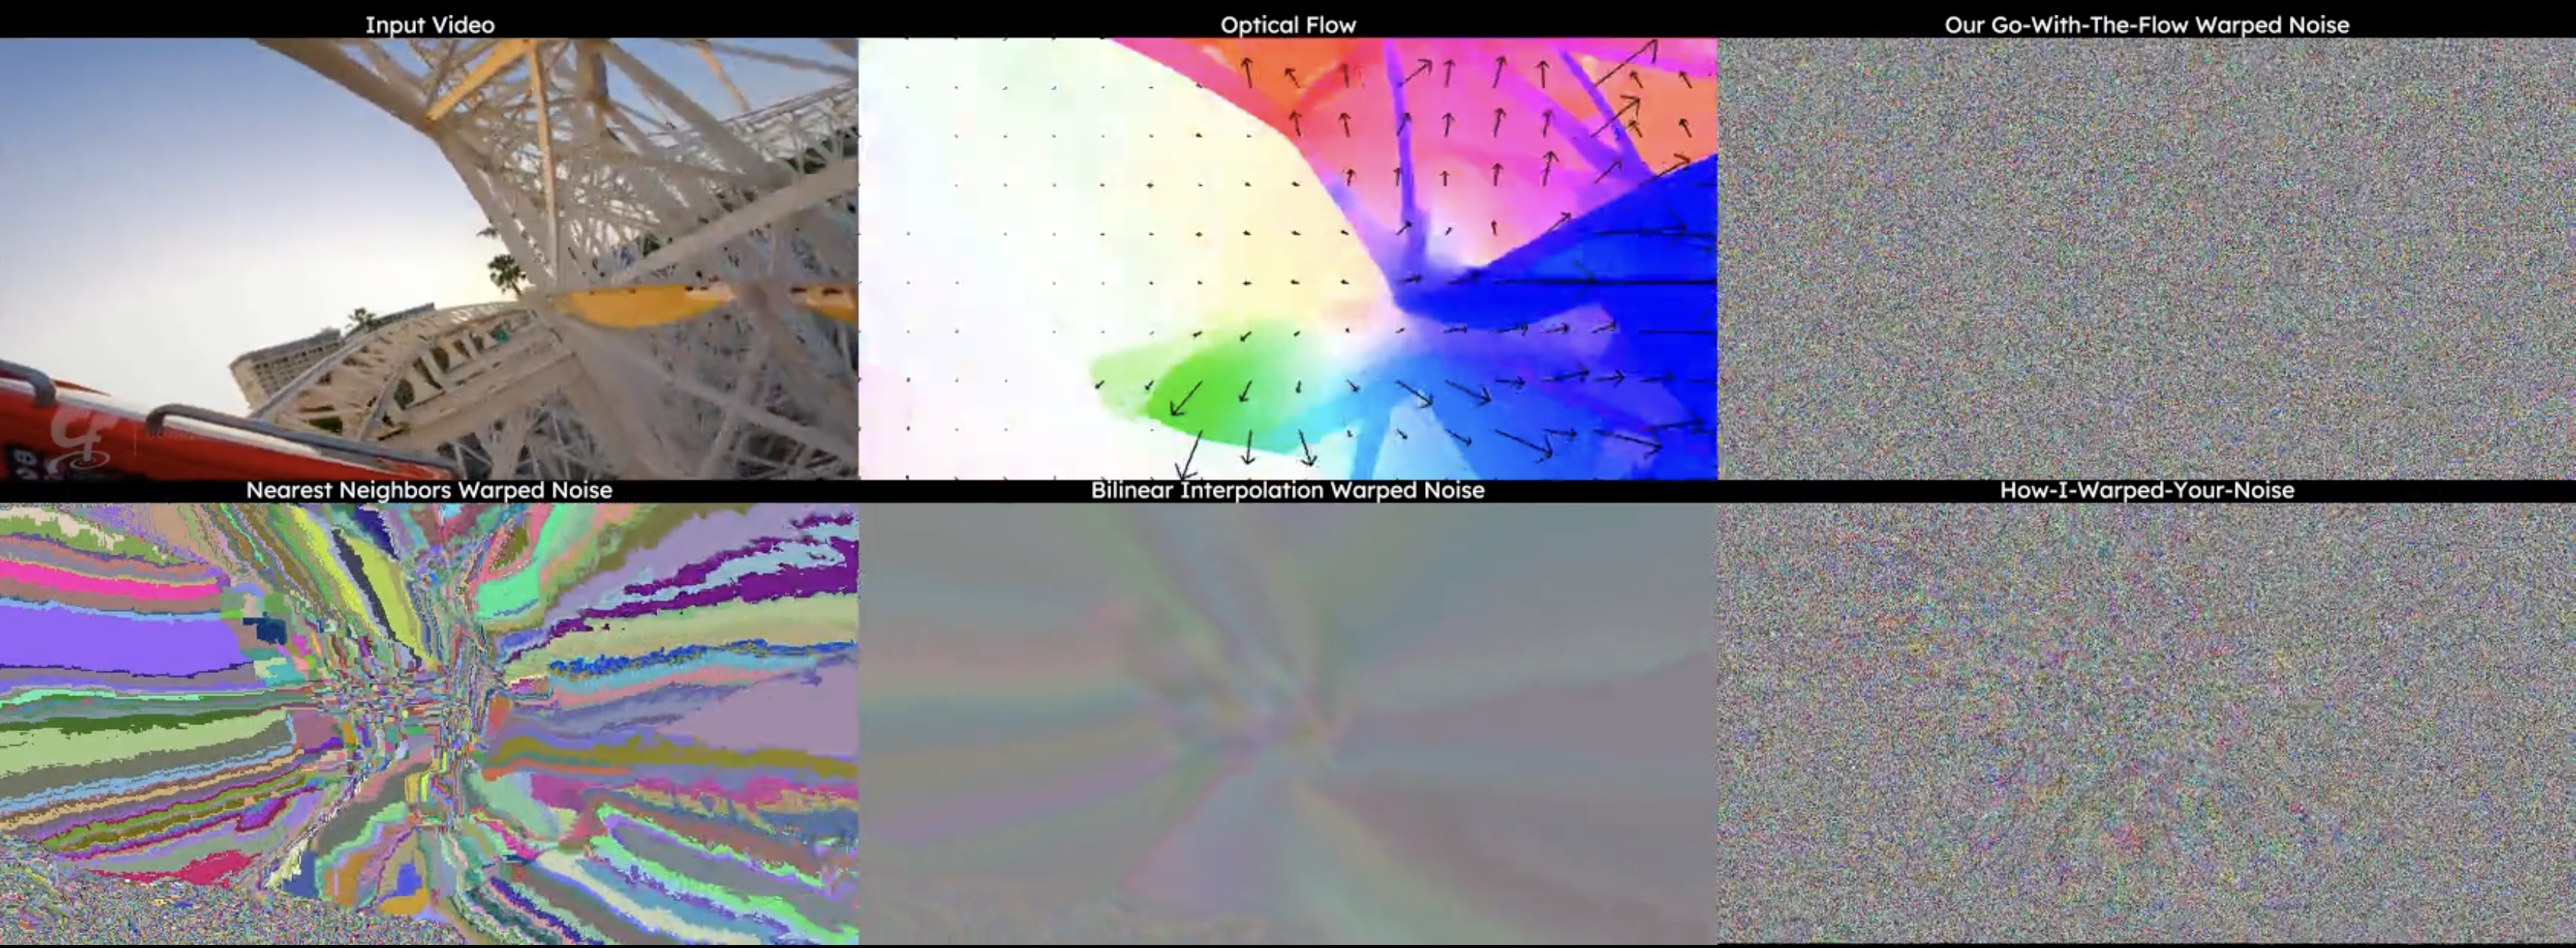
\includegraphics[width=1\linewidth]{fig/nongauss_vis.png}
    \caption{A direct visualization of the noise produced by our noise warping algorithm, HIWYN~\cite{chang2024warped}, bilinear, and nearest neighbor interpolations. The forward movement in this long roller-coaster video forces the noise to expand significantly. Early in the video, the HIWYN baseline produces visibly non-Gaussian results. See the full video on our \href{https://eyeline-research.github.io/Go-with-the-Flow/}{webpage}.}
    \label{fig:supp_warped_noise_flow_vis}
\end{figure*}

\begin{figure}
    \centering
    \includegraphics[width=1\linewidth]{fig/stroller_frame20.png}
    \caption{Using different noise warping algorithms on DeepFloyd~IF for video super-resolution on the DAVIS dataset.}
    \label{fig:supp_davis_deepfloyd}
\end{figure}

\begin{figure}
    \centering
    \includegraphics[width=1\linewidth]{fig/naz_diffrelight_grid11.jpg}
    \caption{Using different noise warping algorithms on DifFRelight for portrait video relighting. }
    \label{fig:supp_diffrelight_noisewarp}
\end{figure}


\section{The advantage of noise warping}

By using noise warping as a condition for motion, we effectively discard all structural information from our input video that cannot be inferred from motion alone. This can be advantageous, as demonstrated in \cref{fig:supp_windmill}. MotionClone does not use optical flow to guide the video trajectory, instead relying on manipulating activations within the diffusion model. As a result, the windmill gains an extra set of arms, whereas our method, which relies solely on motion information from optical flow via warped noise, does not introduce such artifacts.

\section{Comparison to the video diffusion base model without finetuning}

Interestingly, video diffusion models respond to noise warping even without training. In \cref{fig:supp_windmill} the rightmost column, even though the per-frame quality suffers, the flow of the output video still roughly follows the flow of the warped noise. However, because warped noise is statisically distinct from the pure Gaussian noise CogVideoX was trained on, without fine-tuning it can result in visual artifacts.

\section{User study settings and statistics}
\label{sec:supp_user_study}

\cref{fig:supp_user_study_screenshots_statistics} presents our user study questionnaires and statistics for two applications: (1) local object motion control, and (2) turnable camera movement video generation. Our questions focus on users' overall subjective preference, controllability, and temporal consistency.

\section{Model Agnostic}


Our method is data- and model-agnostic. It can be used to add motion control to arbitrary video diffusion models by only processing the noise sampling during fine-tuning. For example, it also works with AnimateDiff \cite{guo2024animatediff} fine-tuned on the WebVid dataset~\cite{Bain21} (the weights for this model on our \href{https://github.com/Eyeline-Research/Go-with-the-Flow}{GitHub} page). See its qualitative results in \cref{fig:supp_animatediff_grid}. Since release, the community has also trained a version of Go-with-the-Flow on HunyuanVideo (linked on our \href{https://github.com/Eyeline-Research/Go-with-the-Flow}{GitHub} page). Therefore, our method will generalize to future more advanced video diffusion base model.

\section{Pseudo code}

See \cref{listing:supp_algo_pseudo_code} for our noise warping pseudo code. See our source code and model checkpoints on \href{https://github.com/GoWithTheFlowPaper/gowiththeflowpaper.github.io}{GitHub}.

\begin{figure*}
    \centering
    \includegraphics[width=0.7\linewidth]{fig/windmills.pdf} 
    \caption{
    We show a \cutndrag~animation of a windmill rotating clockwise, next to the derived optical flow, our outputs, a baseline and an ablation. \textbf{Note} that the input video column appears to have two sets of panels because it's being cut and dragged over itself to create rotational motion. \textbf{When using noise warping is better}: Per-frame structural information can poison the result of MotionClone, giving the windmill an extra set of arms - whereas ours only receives motion information from optical flow alone via warped noise (there are no double-windmills in the optical flow patterns). \textbf{Ablation in rightmost column}: warped noise with $\deglevel=.5$ on the CogVideoX base model before we fine-tune it. Because warped noise is statisically distinct from the pure Gaussian noise CogVideoX was trained on, without fine-tuning it can result in visual artifacts. Note how although the per-frame quality suffers here, it still picks up on motion queues from the warped noise (the camera zooms into the windmill).}
    \label{fig:supp_windmill}
\end{figure*}

\begin{figure*}
    \centering
    \begin{subfigure}{.48\linewidth}
    \includegraphics[width=\linewidth]{fig/user_study_screenshot_1.png}
    \subcaption{User study interface and questions for local object motion control, corresponding to ~\cref{fig:comparisons_video_diffusion_object_motions} in the main paper.}
    \end{subfigure}
    \hfill
    \begin{subfigure}{.48\linewidth}
    \includegraphics[width=\linewidth]{fig/user_study_screenshot_2.png}
    \subcaption{User study interface and questions for turnable camera movement video generation, corresponding to ~\cref{fig:comparisons_video_diffusion_turning_object} in the main paper.}
    \end{subfigure}
    \\[12pt]
    \begin{subfigure}{0.48\linewidth}
    \centering
    \includegraphics[width=.7\linewidth]{fig/user_study_1_statistics_1.png}
    \subcaption{User study statistics for local object motion control on the first question ``\textit{Which video is the best overall?}''}
    \end{subfigure}
    \hfill
    \begin{subfigure}{0.48\linewidth}
    \centering
    \includegraphics[width=.7\linewidth]{fig/user_study_1_statistics_2.png}
    \subcaption{User study statistics for local object motion control on the second question ``\textit{Which video best aligns with the user intent for controlling the object movement based on the input?}''}
    \end{subfigure}
    \\[12pt]
    \begin{subfigure}{0.48\linewidth}
    \centering
    \includegraphics[width=.7\linewidth]{fig/user_study_1_statistics_1.png}
    \subcaption{User study statistics for local object motion control on the third question ``\textit{Which video best preserves the intended camera movement from the input?}''}
    \end{subfigure}
    \hfill
    \begin{subfigure}{0.48\linewidth}
    \centering
    \includegraphics[width=.7\linewidth]{fig/user_study_1_statistics_1.png}
    \subcaption{User study statistics for local object motion control on the fourth question ``\textit{Which video maintains the most consistent and stable motion throughout?}''}
    \end{subfigure}
    \\[12pt]
    \begin{subfigure}{0.48\linewidth}
    \centering
    \includegraphics[width=0.7\linewidth]{fig/user_study_2_statistics_1.png}
    \subcaption{User study statistics for motion transfer on the first question ``\textit{Which video has better overall quality?}''}
    \end{subfigure}
    \caption{User study questionnaires screenshots and statistics. For all the questions of both applications, our method (the rightmost bar plot) significantly wins the most user preferences.}
    \label{fig:supp_user_study_screenshots_statistics}
\end{figure*}

% \begin{figure*}
%     \centering
%     \includegraphics[width=1\linewidth]{fig/animatediff.jpg}
%     \caption{Fine-tuning AnimateDiff with our warped noise flow. All rows share the same movements, and all columns share the same text prompts. The first column is the reference video providing the flow to warp the noise in column 2, which is then used to diffuse all videos to the right. Please zoom in to see the captions for each row (input videos driving movement and warping noise via optical flow) and each column (text prompt for each video cell). Refer to our project video to see these in animation form.}
%     \label{fig:supp_animatediff_grid}
% \end{figure*}

\begin{figure*}
    \centering
    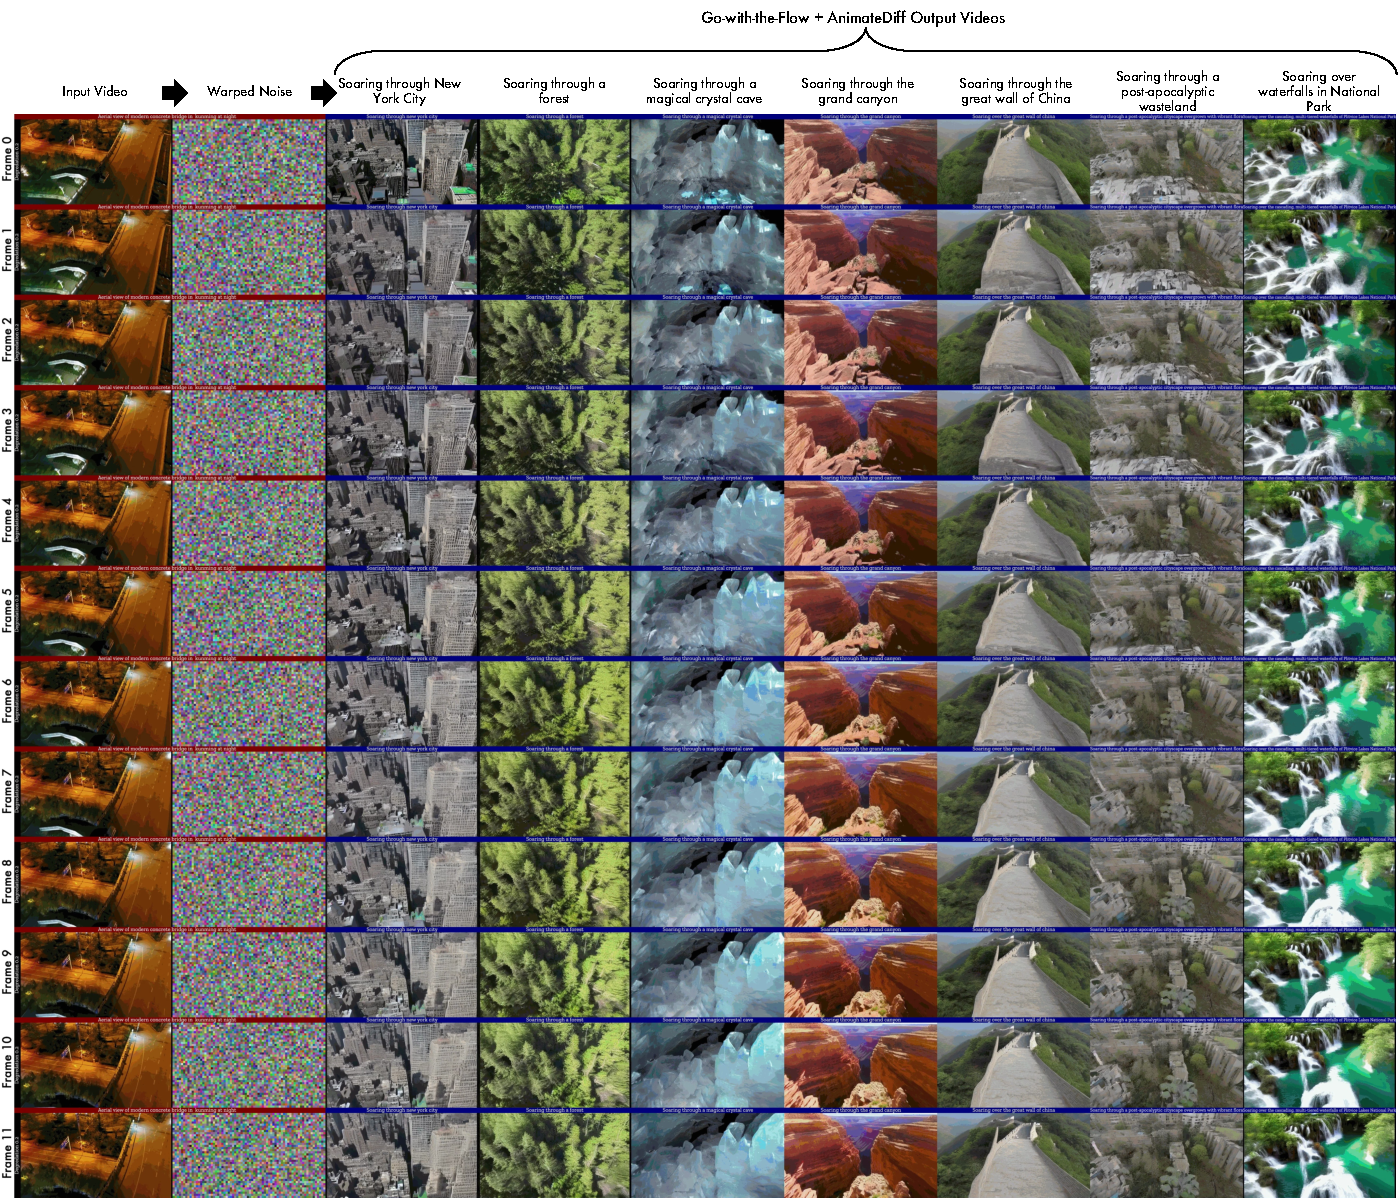
\includegraphics[width=1\linewidth]{fig/AnimateDiffAnimation.pdf}
    \caption{Fine-tuning AnimateDiff with our warped noise flow. We used Go-with-the-Flow to fine-tune AnimateDiff T2V, and display the results above. The input video is on the left, and from that video we derive warped noise which is used to initialize AnimateDiff on the columns to its right with different text prompts.}
    \label{fig:supp_animatediff_grid}
\end{figure*}

\begin{figure*}
\begin{lstlisting}
def warp_noise(prev_frame, cur_frame, prev_noise, prev_weight):

    height, width, _ = prev_frame.shape

    flow = optical_flow(prev_frame, cur_frame) # Agnostic to the optical flow algorithm
    backwards_flow = -flow # A cheap approximation of optical_flow(cur_frame, prev_frame)

    expansion_noise    = zeros(height, width)
    contraction_noise  = prev_noise.copy()

    expansion_mask     = ones (height, width, type=bool)
    contraction_mask   = zeros(height, width, type=bool)

    for x in range(width): for y in range(height):
        dx, dy = flow[x,y]
        if 0 <= x+dx <= width-1 and 0 <= y+dy <= height-1:
            # This particle stays in bounds
            expansion_mask  [x+dx, y+dx] = False
            contraction_mask[x   , y   ] = True  # Contraction mask is True where 

    for x in range(width): for y in range(height):
        if expansion_mask[x, y]:
            dx, dy = backwards_flow[x,y]
            expansion_noise [x, y] = prev_noise[x+dx, y+dy]

    # We've decided which source pixels are involved in contraction and expansion now
    contraction_noise &= contraction_mask
    expansion_noise, contraction_noise, cur_weight = jointly_regaussianize_and_rebalance_weights(
        expansion_noise, contraction_noise, prev_weight
    ) # Regaussianize all noise values here, and divide the weights by the number of pixels in each bin

    contraction_weight = zeros(height, width)
    for x in range(width): for y in range(height):
        if contraction_mask[x, y]:
            # Contraction treats the noise pixels as particles, each moving from the source to the
            # destination with this flow
            dx, dy = flow[x,y]
            # Contraction is a weighted sum of source pixels to a destination pixel
            pixel_weight = cur_weight[x, y]
            # Sum all the source noise pixels that contract to the same destination
            contraction_noise [x+dx, y+dy] += prev_noise[x, y] * pixel_weight
            # When we multiply a noise pixel by a weight, the variance changes by that weight squared
            contraction_weight[x+dx, y+dy] += pixel_weight ** 2 
    contraction_noise /= sqrt(contraction_weight) # Adjust the variance of the summed contracted noise

    # Mixing contraction and expansion noises with their respective masks
    cur_noise = contraction_noise & contraction_mask + expansion_noise & expansion_mask

    return cur_noise, cur_weight
\end{lstlisting}
\caption{Our noise warping pseudo code.}
\label{listing:supp_algo_pseudo_code}
\end{figure*}


\end{document}
